%%%%%%%%%%%%%%%%%%%%%%%%%%%%
% Prototype Implementation %
%%%%%%%%%%%%%%%%%%%%%%%%%%%%

\chapter{Prototyp-Implementierung}
\label{chapter:prototype}

Um den im Kapitel \ref{chapter:interactive-approach} vorgestellten Ansatz für das interaktive Layout von Diagrammen und insbesondere die neu eingeführten Mechanismen für die Interaktion zu validieren, wurde in Rahmen der Arbeit ein Prototyp entwickelt. Mit der Beschreibung des Prototyps beschäftigt sich dieses Kapitel. Im Abschnitt \ref{sec:technologies} wird auf die gewählten Technologien eingegangen. Die Benutzeroberfläche und die unterstützten Funktionen werden im Abschnitt \ref{sec:functions} vorgestellt. Schließlich wird im Abschnitt \ref{sec:architecture} die Architektur des Prototyps thematisiert und einzelne Komponenten beschrieben.

\section{Technologie}
\label{sec:technologies}

Bevor die Entwicklung des Prototyps begonnen hat, wurde nach verfügbaren Komponenten gesucht, die in dem Prototyp verwendet werden könnten. Der umzusetzende Ansatz weist spezielle \textbf{Mechanismen für die Interaktion} auf (siehe Abschnitt \ref{sec:interaction-mechanisms}), die weder in kommerziellen Anwendungen noch in wissenschaftlichen Arbeiten gefunden wurden. Daher lässt sich für die Interaktion keine bestehende Software-Bibliothek einsetzen und die Umsetzung der Mechanismen der Interaktion bildet einen wesentlichen Teil der Entwicklung des Prototyps.

Des Weiteren wurde der Einsatz einer Bibliothek zum \textbf{Graphzeichnen} bedacht. Da die in diesen Bibliotheken bereitgestellte Algorithmen in der Regel eine automatische Berechnung des Layouts durchführen, ist eine Variierung des Layouts durch den Nutzer nicht möglich (siehe Abschnitt \ref{sec:automatic-layout}). Dies ist ebenfalls der Fall beim dem Einsatz dieser Algorithmen in interaktiven Ansätzen. Insbesondere in dem Pattern-basierten Ansatz aus \cite{Maier12A-Pattern-based} ist deutlich zu erkennen, dass sich das Layout nach der Anwendung eines Algorithmus zum Graphzeichnen auf einen gewählten Teil des Diagramms nicht modifizieren lässt (siehe Abschnitt \ref{subsubsec:pattern-based-approach}). Da die Möglichkeit der Layout-Variierung durch den Nutzer eine wichtige Rolle in dem Ansatz spielt, wurde entschieden, die im Abschnitt \ref{subsec:concrete-layout-algorithms} beschriebene Layout-Algorithmen eigenständig zu implementieren. Da es sich um vereinfachte Algorithmen handelt, wurde der Einfachheit halber zu keinem \textbf{Constraintlöser} gegriffen, der z.B. in \textit{Dunnart} eingesetzt wird (siehe Abschnitt \ref{subsubsec:constraint-based-approaches}) und in Form der Software-Bibliothek \textit{Adaptagrams}\footnote{\url{https://github.com/mjwybrow/adaptagrams}} verfügbar ist. Der Einsatz eines Constraintlösers für einen verallgemeinerten Layout-Algorithmus wird im Abschnitt \ref{subsec:algorithm-generalization} diskutiert.

Es wäre denkbar, das \textbf{Layout-Framework aus \cite{Maier12A-Pattern-based}} als Grundlage für die Umsetzung des Prototyps einzusetzen. Dafür wäre es notwendig, die freie Positionierung einzuschränken, z.B. durch das Einführen von impliziten Layout-Patterns. Weiterhin müssten die in \cite{Maier12A-Pattern-based} vorgestellten allgemeinen Layout-Patterns zusammengefasst und um die Möglichkeit der Variierung erweitert werden. Schließlich müsste eine Unterstützung für die Mechanismen der Interaktion geschaffen werden. Da das Layout-Framework zu der Zeit der Anfertigung dieser Bachelor-Arbeit nicht veröffentlicht wurde, war sein Einsatz ausgeschlossen.

Aufgrund der Konzentration auf die Mechanismen der Interaktion und die Bestandteile der Layout-Berechnung wurde das bearbeitete Modell einfach gehalten, das bereits bei der Vorstellung der konkreten Layout-Algorithmen im Abschnitt \ref{subsec:concrete-layout-algorithms} beschrieben wurde. Deshalb war es nicht notwendig, eine verfügbare Implementierung des \textbf{UML-Metamodells} (z.B. Ecore\footnote{\url{http://www.eclipse.org/modeling/emf}}) zu verwenden.

Da keine Komponenten wiederverwendet werden konnten, wurde eine komplett neue Desktop-Anwendung entwickelt. Es handelt sich um eine native \textbf{Mac OS X Anwendung}, die in der Programmiersprache \textit{Objective-C} entwickelt wurde. Sie verwendet ausschließlich die Standardbibliotheken \textit{Cocoa} und \textit{Quartz} und besitzt keine weiteren Abhängigkeiten.

\section{Funktionen}
\label{sec:functions}

Der Ansatz für das interaktive und diagrammspezifische Layout von Diagrammen wurde in einem prototypischen Werkzeug für die Erstellung von einfachen Klassendiagrammen umgesetzt. Das Werkzeug unterstützt Klassen und Vererbungsrelationen und bietet somit die Möglichkeit, Vererbungshierarchien von Klassen zu modellieren.

Die Benutzeroberfläche des Werkzeugfensters ist in zwei rechteckige Bereiche aufgeteilt. Links befindet sich die Sidebar mit Bedienungselementen und rechts der Canvas, in dem das modellierte Diagramm abgebildet wird. Die Sidebar besteht aus einer Palette mit Icons für das Hinzufügen von Klassen und Vererbungsrelationen, einem Button für das Zurücksetzen des modellierten Diagramms und einer Auswahl des verwendeten Layout-Algorithmus. Die Benutzeroberfläche der Anwendung wird mit Hilfe eines Screenshots in Abbildung \ref{fig:prototype-screenshot} veranschaulicht.

\begin{figure}[hbt]
    \centering
    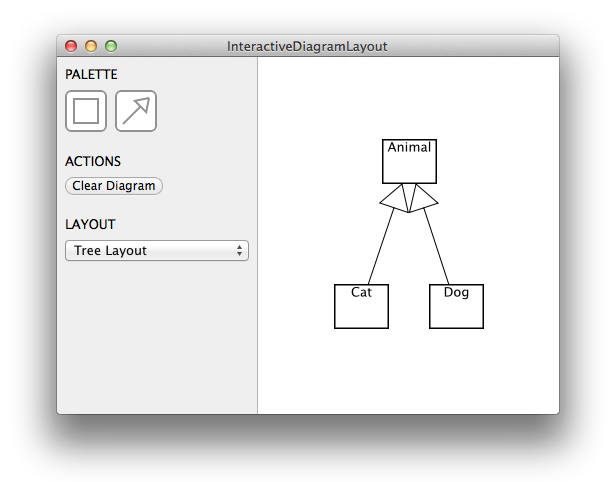
\includegraphics[scale=0.6]{resources/prototype-screenshot}
    \caption{Ein Screenshot des prototypischen Werkzeugs}
    \label{fig:prototype-screenshot}
\end{figure}

\subsection{Unterstützte Aktionen}

Der Prototyp unterstützt die grundlegenden Aktionen, die erforderlich sind, um ein Diagramm modellieren zu können. Insbesondere handelt es sich um die wichtigsten Bearbeitungsaktionen, die im Abschnitt \ref{subsec:edit-actions} vorgestellt wurden. Die einzelnen Aktionen werden im Folgenden aufgelistet und kurz beschrieben:

\begin{itemize}
    \item \textbf{Hinzufügen einer Klasse} Eine neue Klasse kann mit Hilfe von \enquote{Drag and Drop} dem Diagramm hinzugefügt werden, indem das linke Icon in der Palette angeklickt und in den Canvas gezogen wird. Nachdem der Mauszeiger den Canvas erreicht, wird die Klasse hinzugefügt, was durch einen Platzhalter gekennzeichnet wird. Danach wandelt die Aktion in eine Verschiebungsaktion um (siehe unten) und die Klasse kann an eine gewünschte Position verschoben werden.
    \item \textbf{Umbenennen einer Klasse} Durch einen Doppelklick und das Eintragen eines Namens in das angezeigte Textfeld kann eine Klasse im Diagramm umbenannt werden. Aus zeitlichen Gründen konnte die Anpassung der Größe der Klassen nach der Änderung ihren Namen nicht implementiert werden.
    \item \textbf{Verschiebung einer Klasse} Die Position einer Klasse im Diagramm kann durch den Nutzer geändert werden, indem die Klasse mit Hilfe des Mechanismus der temporären Schicht (siehe Abschnitt \ref{subsec:temporary-layer-mechanism}) verschoben wird. Dabei wird das Layout durch die ausgewählte Layout-Engine berechnet (siehe Abschnitt \ref{subsec:supported-layout-methods}).
    \item \textbf{Erzeugen einer Vererbungsrelation zwischen zwei Klassen} Durch das Anklicken des rechten Icons in der Palette und das Ziehen eines Pfeils zwischen zwei Klassen im Diagramm wird eine Vererbungsrelation erstellt. Alternativ kann neben dem Anklicken des Icons auch die Taste \texttt{CTRL} gedrückt werden. Wenn der Nutzer versucht, eine semantisch ungültige Vererbungsrelation zu erstellen (z.B. einen Vererbungszyklus oder eine Mehrfachvererbung\footnote{Die Mehrfachvererbung ist ein gültiges Konstrukt in Klassendiagrammen der Notationssprache UML, wird aber in meisten objekt-orientierten Sprachen nicht unterstützt \cite{ArlowNeustadt05UML-2-and-the-Unified}. Für die Zwecke des Prototyps wird sie nicht zugelassen.}), wird eine Fehlermeldung angezeigt und der Vorgang bricht ab. Nachdem eine Vererbungsrelation erstellt wird und die ausgewählte Layout-Engine die Vererbungsrelationen unterstützt, wird das neu berechnete Layout auf das Diagramm angewendet.
    \item \textbf{Löschen des Inhalts} Da das prototypische Werkzeug keine Möglichkeit der Auswahl von Objekten im Canvas bietet, wird das Löschen von ausgewählten bzw. einzelnen Klassen bzw. Relationen nicht unterstützt. Um trotzdem das Zurücksetzen des Diagramms zu ermöglichen, gibt es für diese Funktion ein Button in der Sidebar.
\end{itemize}

Die Funktionsweise der beschriebenen Aktionen ist in einem Video unter dem Pfad \texttt{Prototype/\-Videos\-/Actions-De\-mo.mov} auf der unter Anhang \ref{chapter:dvd} eingereichten DVD veranschaulicht.

Die implementierten Aktionen sind für die Validierung des umgesetzten Konzepts und die Vorbereitung von Aufgaben für eine Nutzerstudie ausreichend, dennoch ist das prototypische Werkzeug nicht produktiv einsetzbar. Das liegt zum einen auf der starken Einschränkung der Notation der Klassendiagramme und zum anderen auf der ausschließlichen Unterstützung von grundlegenden Aktionen. Die möglichen Erweiterungen des Prototyps werden im Abschnitt \ref{subsec:implementation-of-importent-actions} diskutiert.

\subsection{Unterstützte Layout-Methoden}
\label{subsec:supported-layout-methods}

Der Prototyp unterstützt beide konkreten Layout-Algorithmen aus dem Abschnitt \ref{subsec:concrete-layout-algorithms}, wobei der Algorithmus für das horizontale Layout als ein Zwischenschritt für die Implementierung des Algorithmus für das baumbasierte Layout dient und bei der Layout-Berechnung keine Relationen berücksichtigt.

Der aktuelle Algorithmus kann in der Sidebar ausgewählt werden und wird für die Layout-Berechnung im Diagramm verwendet. Außerdem wird bei der Änderung des Algorithmus ein initiales Layout berechnet, um das Layout des Diagramms in einen validen Zustand zu bringen (siehe Abschnitt \ref{subsec:concrete-layout-algorithms}). Für die Auswahl des Algorithmus können alternativ auch die Tastenkombinationen \texttt{CMD+1} und \texttt{CMD+2} genutzt werden.

\section{Architektur}
\label{sec:architecture}

Der Prototyp wurde in Form einer objekt-orientierten Anwendung implementiert und ist in vier logische Komponenten aufgeteilt: \textit{Layout Engine}, \textit{Dragging Manager}, \textit{Canvas View} und \textit{Application}. Die Abhängigkeiten zwischen den Hauptkomponenten sind in Abbildung \ref{fig:main-components} in Form eines Paketdiagramms dargestellt. Zu den Verantwortlichkeiten der Komponente \textit{Layout Engine} gehört u.a. die Beschreibung des Metamodells, die Verarbeitung der Nutzer-Aktionen und vor allem die Durchführung der Layout-Berechnung. Durch die Komponente \textit{Dragging Manager} wird eine abstrahierte Schnittstelle für die \enquote{Drag and Drop} Operation bereitgestellt. Die Darstellung und Interaktion mit dem Diagramm im Canvas wird in der Komponente \textit{Canvas View} realisiert. Schließlich werden die genannten Komponenten von der Komponente \textit{Application} zu einer lauffähigen Anwendung zusammengesetzt. Auf die einzelnen Komponenten wird in folgenden Abschnitten eingegangen.

\begin{figure}[hbt]
    \centering
    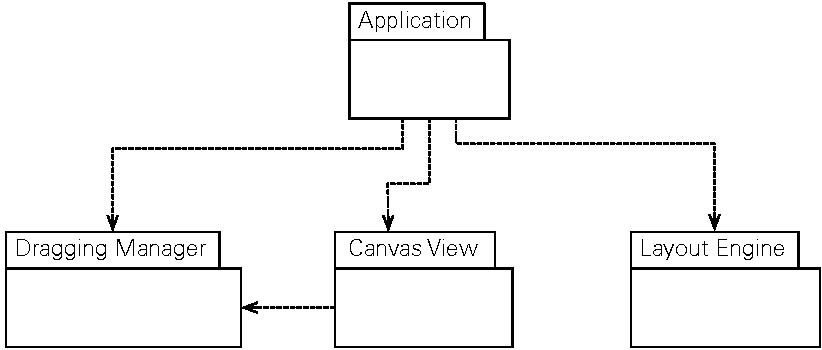
\includegraphics[scale=0.85]{resources/main-components}
    \caption{Eine Übersicht der grundlegenden Komponenten des Prototyps}
    \label{fig:main-components}
\end{figure}

\subsection{Layout Engine}

Die Komponente \textit{Layout Engine} bildet den wesentlichen Teil der Umsetzung des interaktiven Ansatzes aus dem Kapitel \ref{chapter:interactive-approach}. Neben der Beschreibung der Layout-Eigenschaften und des Metamodells für die Diagramme verfügt diese Komponente über die Verwaltung von Layout-Patterns, Erstellung und Verarbeitung von Layout-Ereignissen und schließlich stellt sie die Funktion der Layout-Berechnung zur Verfügung. Aufgrund der Komplexität wurde \textit{Layout Engine} in folgende Unterkomponenten aufgeteilt: \textit{Geometry}, \textit{Diagram}, \textit{Layout}, \textit{Patterns}, \textit{Events} und \textit{Engines}. Eine Übersicht der Unterkomponenten und deren Beziehungen wird in Form eines Paketdiagramms in Abbildung \ref{fig:layout-engine-subcomponents} gegeben.

\begin{figure}[hbt]
    \centering
    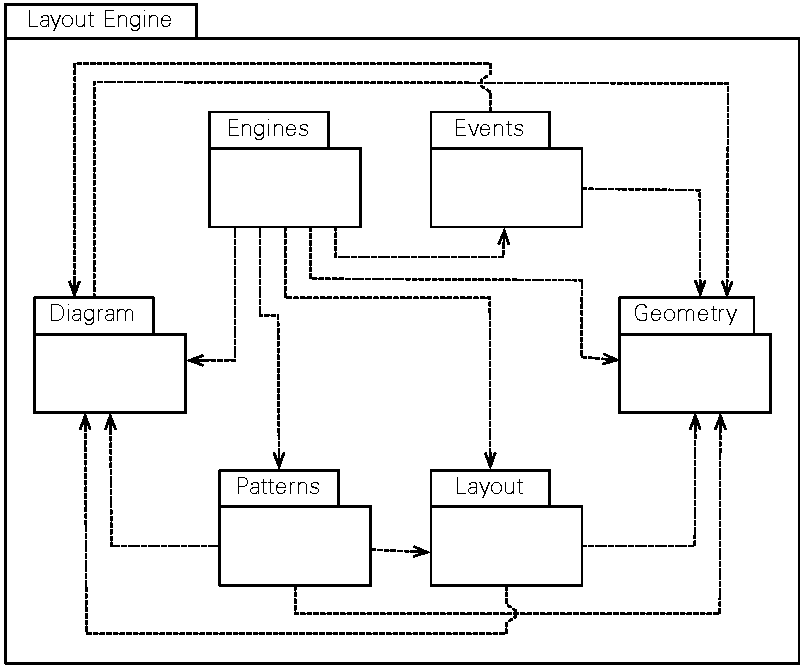
\includegraphics[scale=0.85]{resources/layout-engine-subcomponents}
    \caption{Eine Übersicht der Unterkomponenten der Komponente \textit{Layout Engine}}
    \label{fig:layout-engine-subcomponents}
\end{figure}

\subsubsection{Geometry}

Die Komponente \textit{Geometry} stellt die grundlegenden \textbf{geometrischen Datentypen} wie Punkt, Größe, Rechteck und Linie und für diese ausgelegte \textbf{geometrische Funktionen} bereit. Die neu eingeführten Datentypen unterscheiden sich von den entsprechenden Datentypen aus der Standardbibliothek wie \texttt{NSPoint}, \texttt{NSSize} und \texttt{NSRect} darin, dass die Werte in ganzen Zahlen angegeben werden und dass die Position des Rechtecks seinen Mittelpunkt darstellt. Durch die letztere Eigenschaft wird die Angabe der Positionen mit Hilfe des Mittelpunktes ermöglicht. Außerdem werden die Positionen in zentrierten Koordinaten angegeben, was die Umsetzung des impliziten Patterns zur Zentrierung des Diagramm-Inhalts fördert (siehe Abschnitt \ref{subsubsec:centering-of-diagram-content}) und die relative Layout-Berechnung vereinfacht. Da in \textit{Cocoa} und insbesondere in der für die grafische Repräsentation verantwortlichen Klasse \texttt{NSView} der Koordinatenursprung standardmäßig in der linken unteren Ecke liegt, war es notwendig eine Umrechnung der beiden Koordinatensysteme zu implementieren. In Abbildung \ref{fig:coordinates-conversion} ist der Sachverhalt illustriert, wobei die zentrierten Koordinaten blau, die Standardkoordinaten rot und das Referenzrechteck schwarz dargestellt sind.

\begin{figure}[hbt]
    \centering
    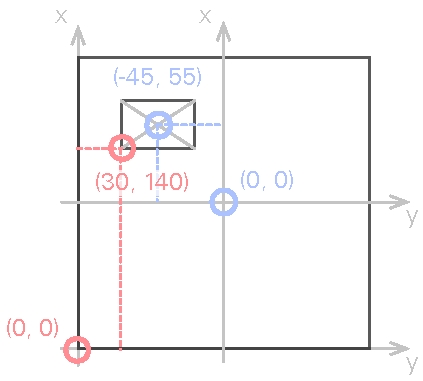
\includegraphics{resources/coordinates-conversion}
    \caption{Ein Beispiel der Koordinatenumrechnung für ein rechteckiges Objekt}
    \label{fig:coordinates-conversion}
\end{figure}

\subsubsection{Diagram}
\label{subsubsec:component-diagram}

% Präfix "IDL" erklären

% aus zeitlichen Gründen wurde die Semantik nicht tiefgründig ausgearbeitet und wurde der weiteren Forschung überlassen
% kein Metamodell
% keine Unterscheidung der abstrakten und konkreten Syntax

% IDLEdge -> gerichtete Kanten mit max. einem Elternknoten (z.B. Vererbung in Klassendiagrammen) -> Diagramm ist also azyklisch

\subsubsection{Layout}

\subsubsection{Patterns}

% nur expliziten
% wie werden die impliziten Patterns im Prototypen implementiert -> durch die konkreten IDLLayoutEngine's
% Wiederverwendung, Komposition in IDLTShapePattern

\begin{figure}[hbt]
    \centering
    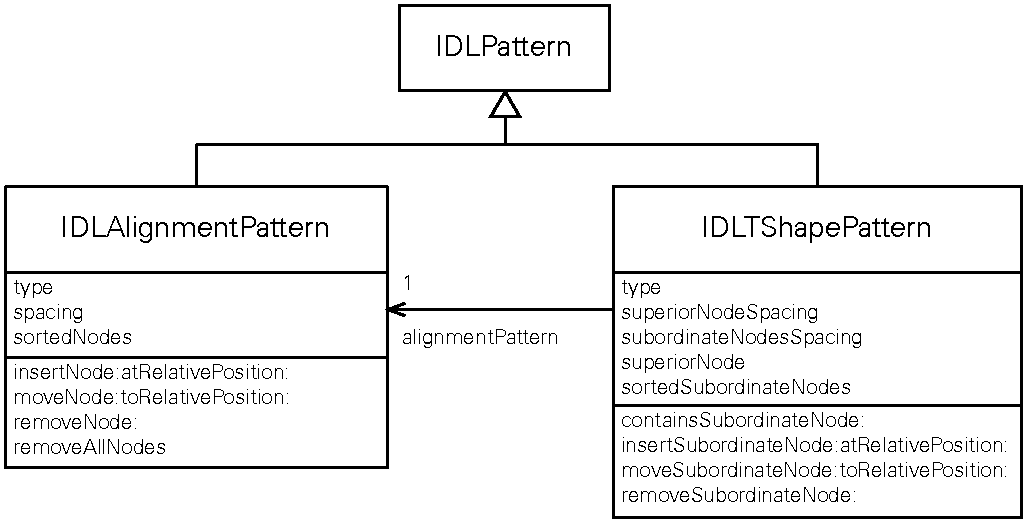
\includegraphics[width=\textwidth]{resources/layout-patterns-implementation}
    \caption{}
    \label{fig:layout-patterns-implementation}
\end{figure}

\subsubsection{Events}

% Löschen nur im Modell, kein UI für die Auswahl

\subsubsection{Engines}

% IDLLayoutEngine & Subclasses (bzw. unterstützte Layout-Engines)

% IDLLayoutEngine besitzt intern Referenzen auf den Inhalt des Diagramms und muss daher mit dem Diagramm synchronisiert werden (manuell) mit s.g. Layout-Events

% Löschen eines (oder mehreren Elementen) im Prototypen nicht unterstützt, nur hinzufügen und "rausfahren"

\subsection{Canvas View}
\label{subsec:canvas-view}

% Animation der Layout-Übergängen
% - implizite Core Animation Animation
% - Überführen von mehreren Animationen mit POP => wichtiger in Multi-Touch-Umgebung, bei Desktop nur ein Mauszeiger, keine parallele Aktionen

% Vergrößerung des Fensters -> Zentrierung des Inhalts (durch die Umrechnung)

% Berechnung der Start- und Endpunkte der Kanten anhand von Eigenschaften der Knoten (siehe OmniGraffle)

\subsection{Dragging Manager}

% Drag and Drop

\subsection{Application}
